\documentclass[tikz]{standalone}
\usepackage{bm}
\begin{document}
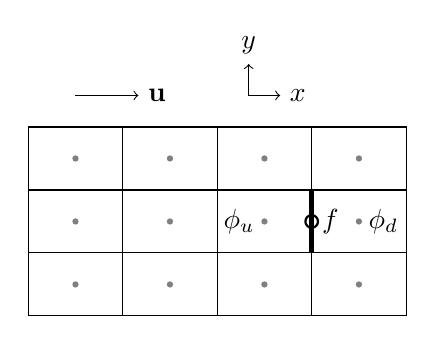
\begin{tikzpicture}[
  scale=0.4,
  cpnt/.style={fill=gray},
]

\draw (0,0) rectangle (12,6);
\draw (3,0) -- (3,6);
\draw (6,0) -- (6,6);
\draw (9,0) -- (9,6);
\draw (0,2) -- (12,2);
\draw (0,4) -- (12,4);

\draw [->] (1.5,7) -- (3.5,7) node [right] {$\mathbf{u}$};
\draw [ultra thick] (9,2) -- (9,4);
\draw [thick] (9,3) circle [radius=0.2] node [anchor=west] {$f$};

\path [cpnt] (1.5,1) circle [radius=0.1];
\path [cpnt] (4.5,1) circle [radius=0.1];
\path [cpnt] (7.5,1) circle [radius=0.1];
\path [cpnt] (10.5,1) circle [radius=0.1];
\path [cpnt] (1.5,3) circle [radius=0.1];
\path [cpnt] (4.5,3) circle [radius=0.1];
\path [cpnt] (7.5,3) circle [radius=0.1] node [left] {$\phi_u$};
\path [cpnt] (10.5,3) circle [radius=0.1] node [right] {$\phi_d$};
\path [cpnt] (1.5,5) circle [radius=0.1];
\path [cpnt] (4.5,5) circle [radius=0.1];
\path [cpnt] (7.5,5) circle [radius=0.1];
\path [cpnt] (10.5,5) circle [radius=0.1];

\draw [<->] (7,8) node [above] {$y$} -- (7,7) -- (8,7) node [right] {$x$};

\end{tikzpicture}
\end{document}
